\documentclass[a4paper,10pt,uplatex,dvipdfmx]{jsarticle}


% 数式
\usepackage{amsmath,amsfonts}
\usepackage{bm}
% 画像
\usepackage[dvipdfmx]{graphicx}
\usepackage{here}
% program
\usepackage{color}
\usepackage{listings, jlisting}
\input{listings-glsl.prf}
% 枠付き
\usepackage{ascmac}

\lstset{
 language={C++},%言語の指定
%  backgroundcolor={\color[gray]{.85}},%背景色と透過度
 basicstyle={\ttfamily},%書体の指定
 identifierstyle={\small\color[rgb]{0.8,0.5,0}},%キーワードでない文字の書体
 commentstyle={\small\itshape\color[rgb]{0,0.3,0}},%注釈の書体
 keywordstyle={\small\bfseries\color[rgb]{0,0.5,1}},%キーワード(int, ifなど)の書体指定
 ndkeywordstyle={\small},%
 stringstyle={\small\ttfamily\color[rgb]{1,0.5,0}},%文字列
 frame={tb},%枠縁(leftline,topline,bottomline,lines,trBL,shadowbox, single)
 breaklines=true,%折り返し(自動改行)
 breakindent = 10pt,  %自動改行後のインデント量(デフォルトでは20[pt])	
 columns=[l]{fullflexible},%
 numbers=left,%行番号表示
 xrightmargin=0zw,%
 xleftmargin=3zw,%
 numberstyle={\scriptsize},%行番号の書体指定
 stepnumber=1,
 numbersep=1zw,%
 lineskip=-0.5ex%
}
\renewcommand{\lstlistingname}{Code} % キャプション名の指定

\begin{document}
\title{アドバンストCG\\ \huge 第5回レポート}
\author{学籍番号:201811411\\ 所属:情報学群情報メディア創成学類\\ 氏名:加藤虎之介}
\date{\today}
\maketitle

\section{実行環境}
\subsection{実行に用いたOS}
macOS Big Sur ver11.3.1

\subsection{プログラム起動時に表示される情報}
\begin{screen}
  OpenGL version: 4.1 ATI-4.4.17\\
  GLSL version: 4.10\\
  Vendor: ATI Technologies Inc.\\
  Renderer: AMD Radeon Pro 5300M OpenGL Engine
\end{screen}

\section{課題A}
\subsection{修正したソースコード}

\subsubsection{Affine Deformationsの実装}
\begin{lstlisting}[caption=affineDeformation]
glm::vec2 rxMeshDeform2D::affineDeformation(const glm::vec2 &v, const glm::vec2 &pc, const glm::vec2 &qc, const double alpha)
{
	// TODO:この部分で 入力頂点座標v と 制御点座標p,q から入力頂点の変形後の座標を計算するコードを書く
	// - 横ベクトル×行列の計算部分はglmのオペレータ*は使わない方がよい(glmは縦ベクトルを前提としている)
	// - Ajを計算してから変形後の座標を計算するのでも,スライドp43の式を直接計算するのでもどちらでもOK
	//   (Ajの前計算は今回は行わないでもよい)
	//
	// - 制御点でループして相対座標を計算するまでのコード例:

	// Ajの逆行列部分の計算
	glm::mat2 WP = glm::mat2(0.f);
	for (size_t k = 0; k < m_iNfix; k++) // 制御点数(m_iNfix)でループを回す
	{
		int i = m_vFix[k]; // 制御点の頂点インデックス

		// 重み
		const glm::vec2 &p = m_vP[i];
		// 固定点と計算点の間の距離に基づく重み
		double dist = glm::length2(p - v);
		float w = (dist > 1.0e-6) ? 1.0f / pow(dist, 2.0f * alpha) : 0.0f;
		// 重心を中心とした制御点の相対座標
		const glm::vec2 p_hat = p - pc;

		WP[0][0] += p_hat.x * w * p_hat.x;
		WP[0][1] += p_hat.y * w * p_hat.x;
		WP[1][0] += p_hat.x * w * p_hat.y;
		WP[1][1] += p_hat.y * w * p_hat.y;
	}

	// 行列式
	double det = glm::determinant(WP);
	// 正則性のチェック
	if (det < 1.0e-6)
	{
		return v;
	}
	// 逆行列の計算
	glm::mat2 invWP = glm::inverse(WP);

	// fa(v)を計算
	glm::vec2 fa = glm::vec2(0.f);
	for (int k = 0; k < m_iNfix; ++k)
	{										 // 制御点数(m_iNfix)でループを回す
		int j = m_vFix[k]; // 制御点の頂点インデックス

		// 重心を中心とした制御点の相対座標
		// 各頂点の座標は配列m_vPとm_vXに格納されている(それぞれ初期形状と変形後の形状)
		const glm::vec2 p_hat = m_vP[j] - pc; // 初期形状での座標
		const glm::vec2 q_hat = m_vX[j] - qc; // 変形後の座標

		// 固定点と計算点の間の距離に基づく重み
		const glm::vec2 p = m_vP[j];
		double dist = glm::length2(p - v);
		float w = (dist > 1.0e-6) ? 1.0f / pow(dist, 2.0f * alpha) : 0.0f;

		// Ajを計算する
		glm::vec2 B = v - pc;
		float A = w * ((B.x * invWP[0].x + B.y * invWP[0].y) * p_hat.x + (B.x * invWP[1].x + B.y * invWP[1].y) * p_hat.y);

		fa += A * q_hat;
	}

	// 変形後の頂点vの座標
	fa += qc;

	return fa;
}
\end{lstlisting}

\subsubsection{Similarity Deformationsの実装}
\begin{lstlisting}[caption=similarityDeformation]
glm::vec2 rxMeshDeform2D::similarityDeformation(const glm::vec2 &v, const glm::vec2 &pc, const glm::vec2 &qc, const double alpha)
{
	// TODO:この部分で 入力頂点座標v と 制御点座標p,q から入力頂点の変形後の座標を計算するコードを書く
	// - 横ベクトル×行列の計算部分はglmのオペレータ*は使わない方がよい(glmは縦ベクトルを前提としている)
	// - μsを先に計算してから変形後の頂点位置を計算
	// - 行列A_iの前計算は今回は行わないでもよい

	// μsを計算
	float ms = 0.0f;
	for (size_t k = 0; k < m_iNfix; k++)
	{
		int i = m_vFix[k];
		const glm::vec2 p = m_vP[i];
		const glm::vec2 p_hat = p - pc;

		// 重みw
		double dist = glm::length2(p - v);
		float w = (dist > 1.0e-6) ? 1.0f / pow(dist, 2.0f * alpha) : 0.0f;

		// μsに加算
		ms += w * (p_hat.x * p_hat.x + p_hat.y * p_hat.y);
	}

	// fs(v)を計算
	glm::vec2 fsv = glm::vec2(0.0f);

	glm::vec2 vecVPc = v - pc;
	glm::mat2 matVPc;
	matVPc[0][0] = vecVPc.x;
	matVPc[0][1] = vecVPc.y;
	matVPc[1][0] = vecVPc.y;
	matVPc[1][1] = -vecVPc.x;
	glm::mat2 trnsMatVPc = glm::transpose(matVPc);

	for (int k = 0; k < m_iNfix; k++)
	{
		int i = m_vFix[k];
		const glm::vec2 p = m_vP[i];
		const glm::vec2 p_hat = p - pc;
		const glm::vec2 q_hat = m_vX[i] - qc;

		// 重みw
		double dist = glm::length2(p - v);
		float w = (dist > 1.0e-6) ? 1.0f / pow(dist, 2.0f * alpha) : 0.0f;

		// 変位行列A
		glm::mat2 matP;
		matP[0][0] = p_hat.x;
		matP[0][1] = p_hat.y;
		matP[1][0] = p_hat.y;
		matP[1][1] = -p_hat.x;

		glm::mat2 A = w * matP * trnsMatVPc;

		// 加算
		fsv += glm::transpose((1.0f / ms) * A) * q_hat;
	}
	// 変形後の頂点vの座標
	fsv += qc;

	return fsv;
}
\end{lstlisting}

\subsubsection{Rigid Deformationsの実装}
\begin{lstlisting}[caption=rigidDeformation]
glm::vec2 rxMeshDeform2D::rigidDeformation(const glm::vec2 &v, const glm::vec2 &pc, const glm::vec2 &qc, const double alpha)
{
	// TODO:この部分で 入力頂点座標v と 制御点座標p,q から入力頂点の変形後の座標を計算するコードを書く
	// - 横ベクトル×行列の計算部分はglmのオペレータ*は使わない方がよい(glmは縦ベクトルを前提としている)
	// - μfを先に計算してから変形後の頂点位置を計算
	// - 行列A_iの前計算は今回は行わないでもよい

	// μfを計算
	// mf = sqrt(A^2 + B^2)とする
	float A = 0.0f;
	float B = 0.0f;
	for (size_t k = 0; k < m_iNfix; k++)
	{
		int i = m_vFix[k];
		const glm::vec2 p = m_vP[i];
		const glm::vec2 p_hat = p - pc;
		const glm::vec2 q_hat = m_vX[i] - qc;

		// 重みw
		double dist = glm::length2(p - v);
		float w = (dist > 1.0e-6) ? 1.0f / pow(dist, 2.0f * alpha) : 0.0f;

		A += w * (q_hat.x * p_hat.x + q_hat.y * p_hat.y);
		B += w * (q_hat.x * -p_hat.y + q_hat.y * p_hat.x);
	}
	const float mf = glm::sqrt(A * A + B * B);

	// fr(v)を計算
	glm::vec2 frv = glm::vec2(0.0f);

	glm::vec2 vecVPc = v - pc;
	glm::mat2 matVPc;
	matVPc[0][0] = vecVPc.x;
	matVPc[0][1] = vecVPc.y;
	matVPc[1][0] = vecVPc.y;
	matVPc[1][1] = -vecVPc.x;
	glm::mat2 trnsMatVPc = glm::transpose(matVPc);

	for (int k = 0; k < m_iNfix; k++)
	{
		int i = m_vFix[k];
		const glm::vec2 p = m_vP[i];
		const glm::vec2 p_hat = p - pc;
		const glm::vec2 q_hat = m_vX[i] - qc;

		// 重みw
		double dist = glm::length2(p - v);
		float w = (dist > 1.0e-6) ? 1.0f / pow(dist, 2.0f * alpha) : 0.0f;

		// 変位行列A
		glm::mat2 matP;
		matP[0][0] = p_hat.x;
		matP[0][1] = p_hat.y;
		matP[1][0] = p_hat.y;
		matP[1][1] = -p_hat.x;

		glm::mat2 A = w * matP * trnsMatVPc;

		// 加算
		frv += glm::transpose((1.0f / mf) * A) * q_hat;
	}

	// 変形後の頂点vの座標
	frv += qc; // ここも書き換えること

	return frv;
}
\end{lstlisting}

\subsection{実行結果}
格子状メッシュかつ、alpha=1.00の条件でプログラムを実行した結果は以下のようになった。
\begin{figure}[H]
  \centering
  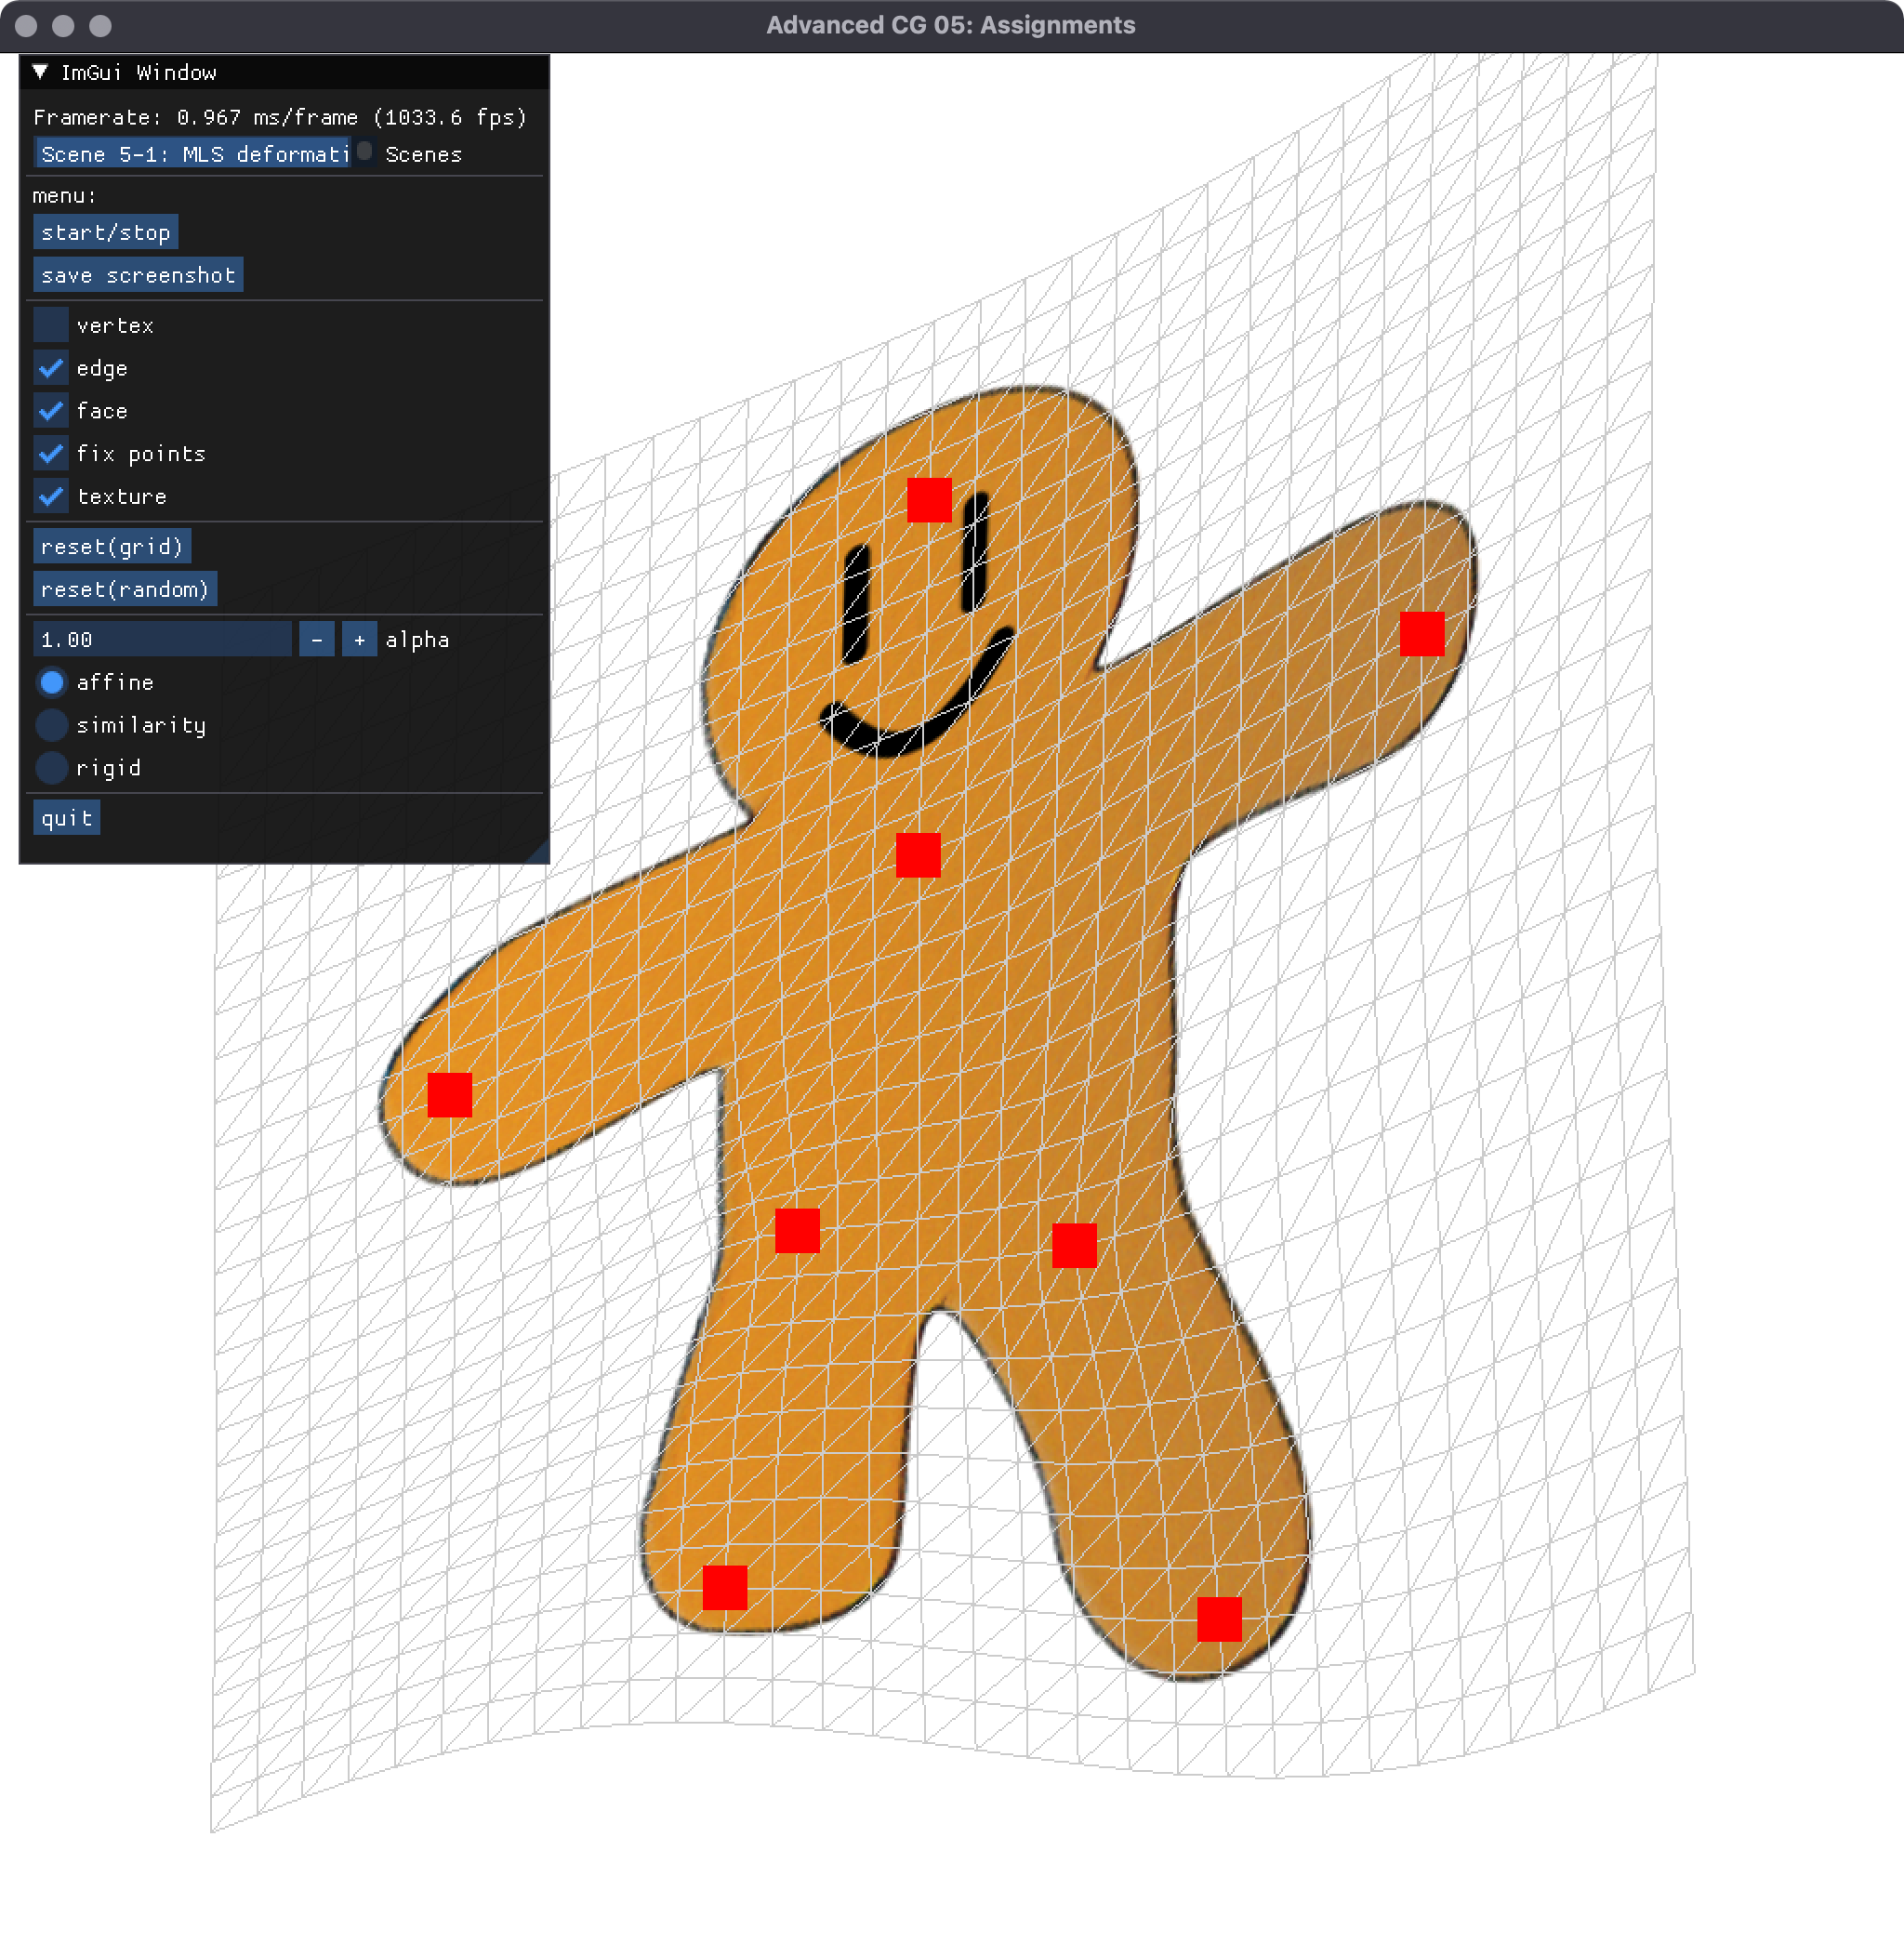
\includegraphics[width=6cm]{./img/affine.png}
  \caption{Affine Deformationの実行結果}

  \vspace{5mm}

  \centering
  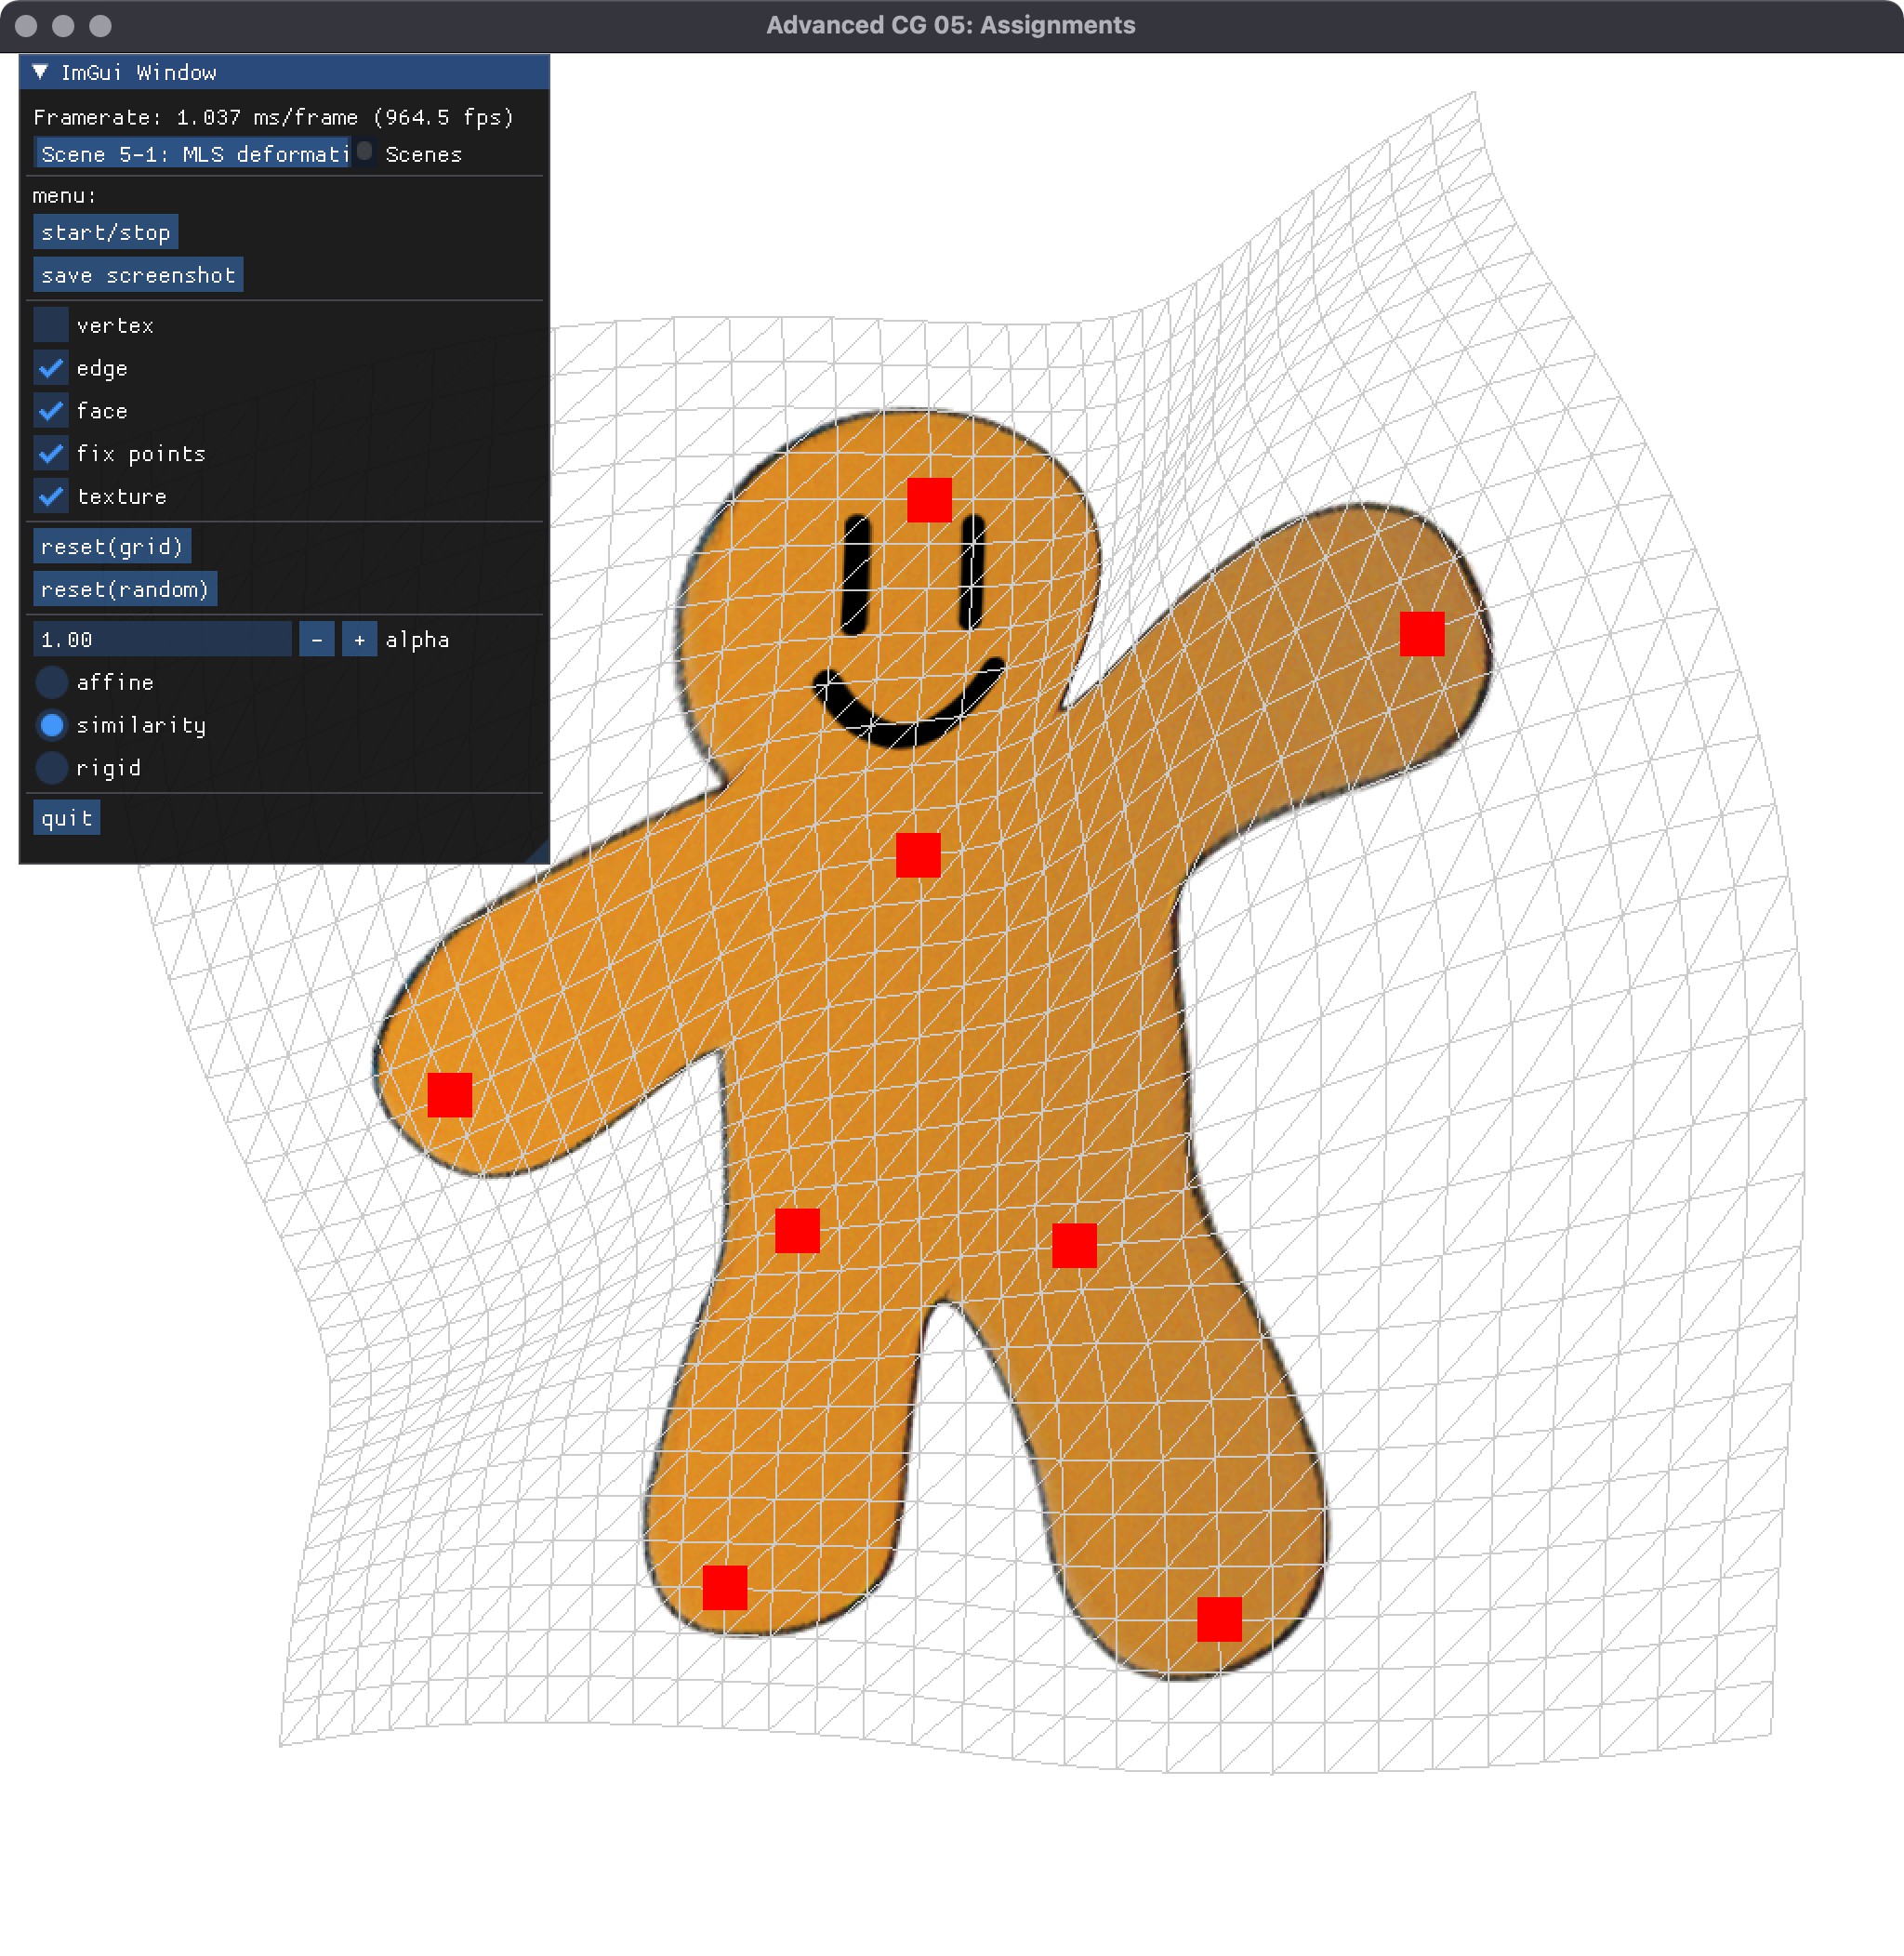
\includegraphics[width=6cm]{./img/similarity.png}
  \caption{Similarity Deformationの実行結果}

  \vspace{5mm}

  \centering
  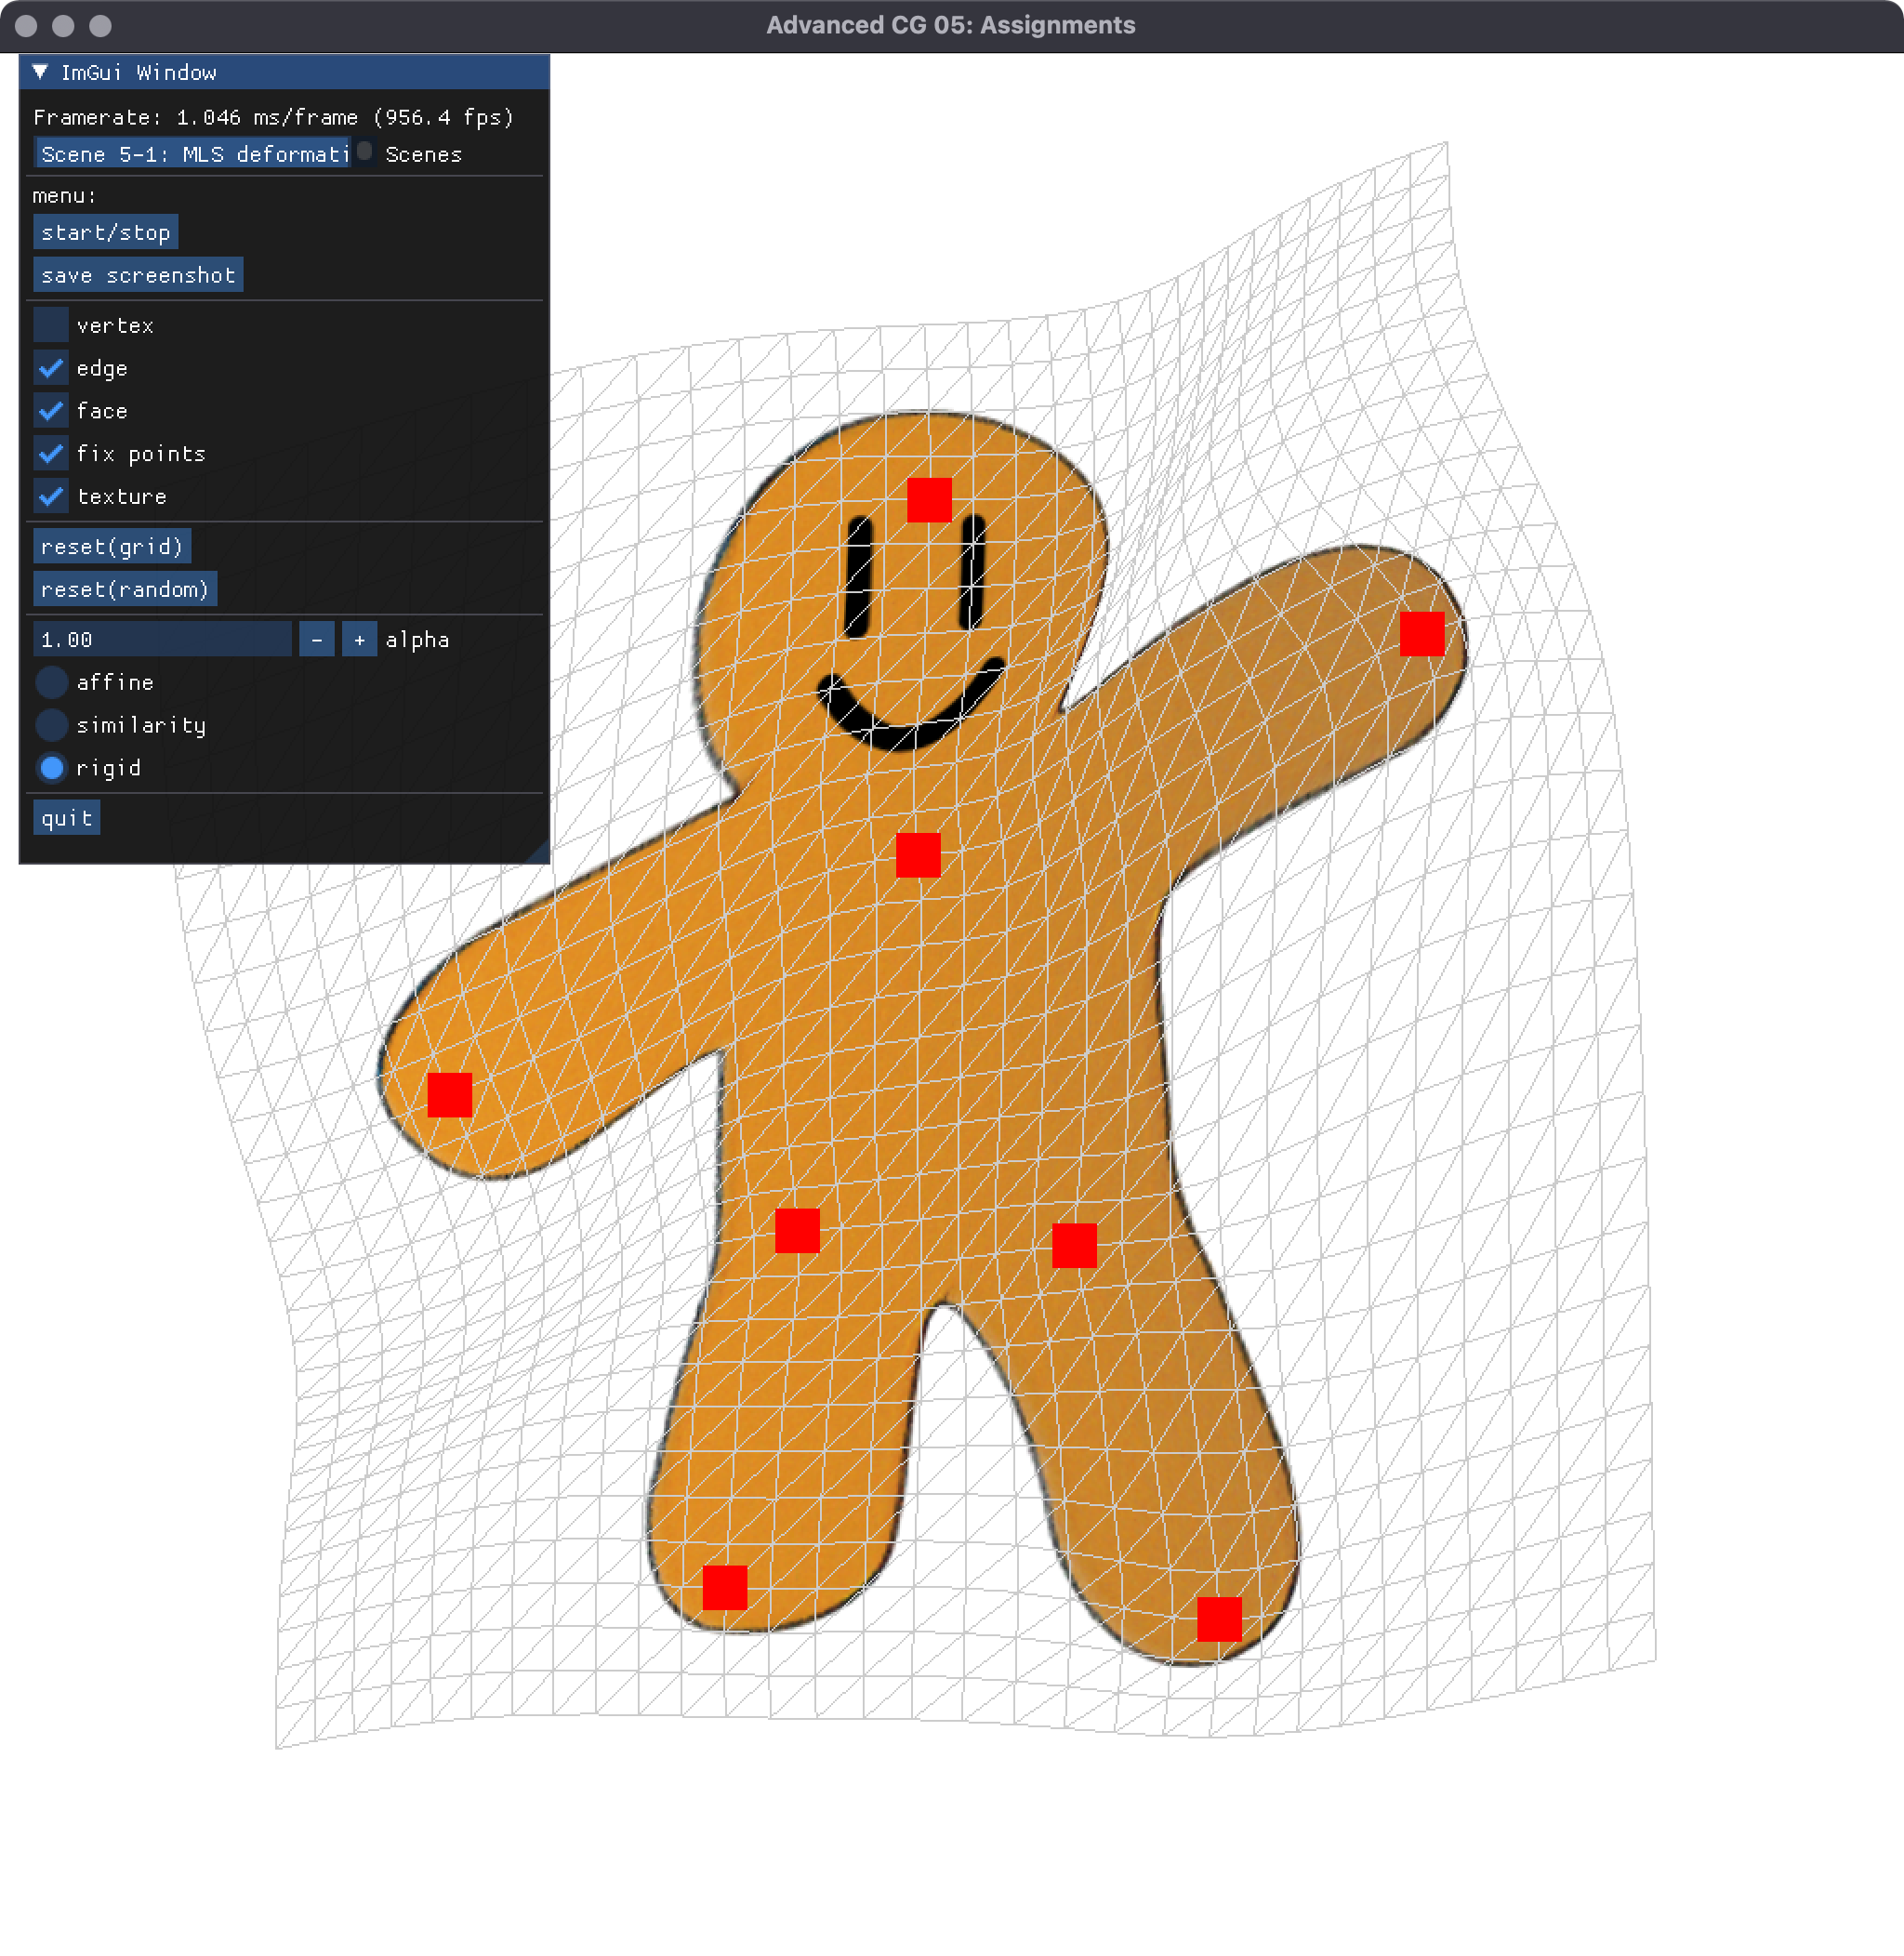
\includegraphics[width=6cm]{./img/rigid.png}
  \caption{Rigid Deformationの実行結果}
\end{figure}

\end{document}